\chapter{Empirische Ist-Analyse des HWG-Formularbestands}
\label{chap:ist_analyse}

Dieses Kapitel widmet sich der systematischen Erhebung und Analyse des bestehenden Formularbestands an der Hochschule für Wirtschaft und Gesellschaft Ludwigshafen (HWG). Ziel ist es, gewachsene Usability-Defizite, Brüche im visuellen Corporate Design sowie Barrierefreiheitsmängel empirisch und quantitativ offenzulegen. Die hieraus gewonnenen Erkenntnisse bilden das empirische Fundament für die anschließende Konzeption des einheitlichen Formular-Standards und der maschinenlesbaren Prüfregeln.

\section{Erhebungsmethodik und Charakterisierung des Formular-Korpus}
\label{sec:methodik_korpus}

Die Bestandsaufnahme basiert auf einer Vollerhebung der zentral im Formular-Management-System Formcycle bereitgestellten Vorlagen. Der erhobene Rohbestand umfasst 49 Formular-Archive (\texttt{.xfp}), aufgeteilt in das Produktivsystem (\texttt{prod}, 15 Vorlagen) sowie das Test- und Entwicklungssystem (\texttt{test}, 34 Vorlagen). Nach Bereinigung von redundanten Sicherungskopien und Zwischenversionen ergab sich ein bereinigtes Kernkorpus von \textbf{34 distinkten Formular-Projekten} mit insgesamt \textbf{49 Workflow-Prozessgraphen}.

Mithilfe eigens entwickelter Analysewerkzeuge wurden die zugrundeliegenden JSON-Modelle (\texttt{.fcp}-Dateien für die Maskenstruktur sowie \texttt{.fcexport}-Dateien für die Prozessketten) automatisiert extrahiert und quantitativ ausgewertet. Zur Erfassung der realen Benutzerschnittstelle wurden zusätzlich von acht Kernformularen gerenderte DOM-Snapshots im HTML-Format erhoben, welche die Einstiegsansicht aus Antragstellenden-Sicht repräsentieren.

\subsection{Klassifikation in funktionale Archetypen}
\label{subsec:archetypen}

Die Analyse offenbart eine enorme strukturelle Spannweite: Die Formulare reichen von schlanken, einseitigen Abfragen mit 30 Elementen bis hin zu hochkomplexen Anträgen mit 424 UI-Elementen und 12 Bildschirmseiten (z.\,B. der Dienstreiseantrag). Inhaltlich lassen sich die Vorlagen in vier funktionale Archetypen unterteilen (siehe Tabelle~\ref{tab:archetypen}):

\begin{table}[htbp]
\centering
\small
\begin{tabularx}{\textwidth}{l>{\raggedright\arraybackslash}Xccc}
\toprule
\textbf{Archetyp} & \textbf{Typische Anwendungsbereiche \& Beispiele} & \textbf{Elemente} & \textbf{Seiten} & \textbf{Anteil} \\
\midrule
\textbf{1. Studierendenprozesse} & Praxisphasen-Anmeldungen (\textit{FB1-GiP-Praktikum}), Notenverbuchung & 114--133 & 2 & 22\,\% \\
\textbf{2. Finanzen, Beschaffung \& Reisen} & Auslagenerstattung, Vergabevermerke, Dienstreiseantrag & 63--424 & 3--12 & 27\,\% \\
\textbf{3. Personalverwaltung (HR)} & Stellen\-ausschreibungen, Vertragsänderungen, Nebentätigkeiten & 110--345 & 2--9 & 24\,\% \\
\textbf{4. Forschung \& Transfer (ZFK)} & Drittmittel-Sprints, Promotionsförderung, Tagungsbeihilfen & 30--419 & 1--10 & 27\,\% \\
\bottomrule
\end{tabularx}
\caption{Funktionale Archetypen der analysierten HWG-Formulare}
\label{tab:archetypen}
\end{table}

\subsection{Empirisches Profil dreier repräsentativer Kernanträge}
\label{subsec:profil_kernantraege}

Um die Bandbreite der existierenden Implementierungsstile zu illustrieren, stellt Tabelle~\ref{tab:vergleich_kernformulare} drei reale Anträge aus unterschiedlichen Fachdomänen dem internen Referenzmuster (\textit{Master-Formular}) gegenüber:

\begin{table}[htbp]
\centering
\scriptsize
\begin{tabularx}{\textwidth}{l*4{>{\raggedright\arraybackslash}X}}
\toprule
\textbf{Prüfdimension} & \textbf{Auslagenerstattung (Prod)} & \textbf{Antrag-Sprints (Test/ZFK)} & \textbf{FB1-Praktikum (Prod)} & \textbf{Master-Formular (Admin)} \\
\midrule
Domäne & Finanzen / Haushalt & Forschung \& Kooperation & Fachbereich 1 / Studium & Zentrale Vorlage \\
Layout-Breite & 700px (starr) & 850px (modern) & 700px (starr) & 700px (starr) \\
Seitenanzahl & 3 Seiten & 1 Seite & 2 Seiten & 1 Seite \\
Header-Banner & HWG-Logo vorhanden & Kein Logo / kein Banner & Kein Logo / kein Banner & HWG-Logo vorhanden \\
Footer-Branding & XIMA-Logo deaktiviert & XIMA-Logo aktiv & XIMA-Logo aktiv & XIMA-Logo deaktiviert \\
Container-Struktur & 4 \texttt{<fieldset>}-Gruppen & 0 Fieldsets (nur \texttt{<div>}) & 2 Fieldsets* & 4 \texttt{<fieldset>}-Gruppen \\
Pflichtfeld-Kennzeichnung & Optischer Stern vorhanden & Optischer Stern vorhanden & Sterne fehlen teilweise & Vollständig mit Stern \\
ARIA-Attribute & \texttt{aria-required} \texttt{="true"} & \texttt{aria-required} \texttt{="true"} & Fehlt teilweise & \texttt{aria-required} \texttt{="true"} \\
IBAN-/PLZ-Validierung & Unvalidierter Freitext & Telefon unvalidiert & Unvalidiert & PLZ unvalidiert \\
Dateiuploads & 4 Uploads ohne Formatangabe & Keine Uploads & 1 Upload* ohne Größenangabe & Keine Uploads \\
Datenschutz (Art. 13) & Kein DSGVO-Hinweis & Kein DSGVO-Hinweis & Kein DSGVO-Hinweis & Im Footer aktiv (\texttt{privacyPolicyShow="1"}) \\
Primär-Button & \texttt{senden} & \texttt{senden} / \texttt{Kritischer Fall} & \texttt{Antrag einreichen} & Keiner (Template-Snippet) \\
Workflow-E-Mail & Bestätigung vorhanden & Bestätigung vorhanden & Bestätigung vorhanden & Keine Workflow-Mail \\
\bottomrule
\end{tabularx}
\caption{Struktureller und ergonomischer Vergleich dreier Kernformulare mit dem Master-Formular (*Die Struktur- und Upload-Werte für FB1-Praktikum beziehen sich auf die gerenderte Einstiegsseite; das Gesamtprojekt umfasst über alle Verzweigungen hinweg 17 Dateiuploads und 20 Fieldset-Container)}
\label{tab:vergleich_kernformulare}
\end{table}

\section{Identifikation zentraler Problemfelder und Heuristik-Audit}
\label{sec:problemfelder}

Der detaillierte Komponenten- und DOM-Vergleich offenbart erhebliche ergonomische und technische Inkonsistenzen, die den Grundsätzen der DIN EN ISO 9241-110, den Richtlinien nach \textcite{bargas2010usable} sowie den WCAG 2.1 widersprechen. Im Folgenden werden die sechs zentralen Problemfelder detailliert analysiert.

\subsection{Problemfeld 1: Layout-Inkonsistenzen und starre Breitenbrüche}
\label{subsec:problem_breiten}

Die quantitative Auswertung aller Vorlagen zeigt eine fundamentale Zerrissenheit des Bestands:
\begin{itemize}
    \item \textbf{700px-Gruppe (53\,\% des Bestands):} Ältere Formulare aus der Personalverwaltung und dem Studierendenservice sowie das interne \textit{Master-Formular} (18 von 34 Vorlagen) sind starr auf eine Maximalbreite von \texttt{700px} fixiert (\texttt{max-width: 700px; min-width: 300px;}). Auf modernen hochauflösenden Monitoren wirkt das Formular wie ein schmaler Fremdkörper; bei horizontalen Mehrfachspalten kommt es zu unschönen Zeilenumbrüchen.
    \item \textbf{850px-Gruppe (47\,\% des Bestands):} Neuere Formulare (insbesondere aus dem Forschungs- und IT-Umfeld, 16 von 34 Vorlagen) nutzen durchgängig eine Maximalbreite von \texttt{850px}.
\end{itemize}
Dieser Generationswechsel ist historisch auf geänderte Voreinstellungen im Formcycle-System zurückzuführen. Da es an einer zentralen Styleguide-Vorgabe fehlte, wechselt die Darstellung für Nutzende innerhalb des Hochschulportals unvorhersehbar, was die \textbf{Erwartungskonformität nach ISO 9241-110} verletzt.

\subsection{Problemfeld 2: Uneinheitliche Corporate Identity und Header-Strukturen}
\label{subsec:problem_ci}

Ein professioneller behördlicher Webauftritt erfordert die verlässliche Wiedererkennung der Institution. Während etablierte Formulare wie die \textit{Auslagenerstattung} über ein gestochen scharfes HWG-Logo im Kopfbereich verfügen, verzichten neuere Anträge (z.\,B. \textit{Antrag auf Förderung Antrag-Sprints}) vollständig auf visuelle Markenanker (siehe Abbildung~\ref{fig:vergleich_header}).

\begin{figure}[htbp]
    \centering
    \begin{subfigure}[b]{0.48\textwidth}
        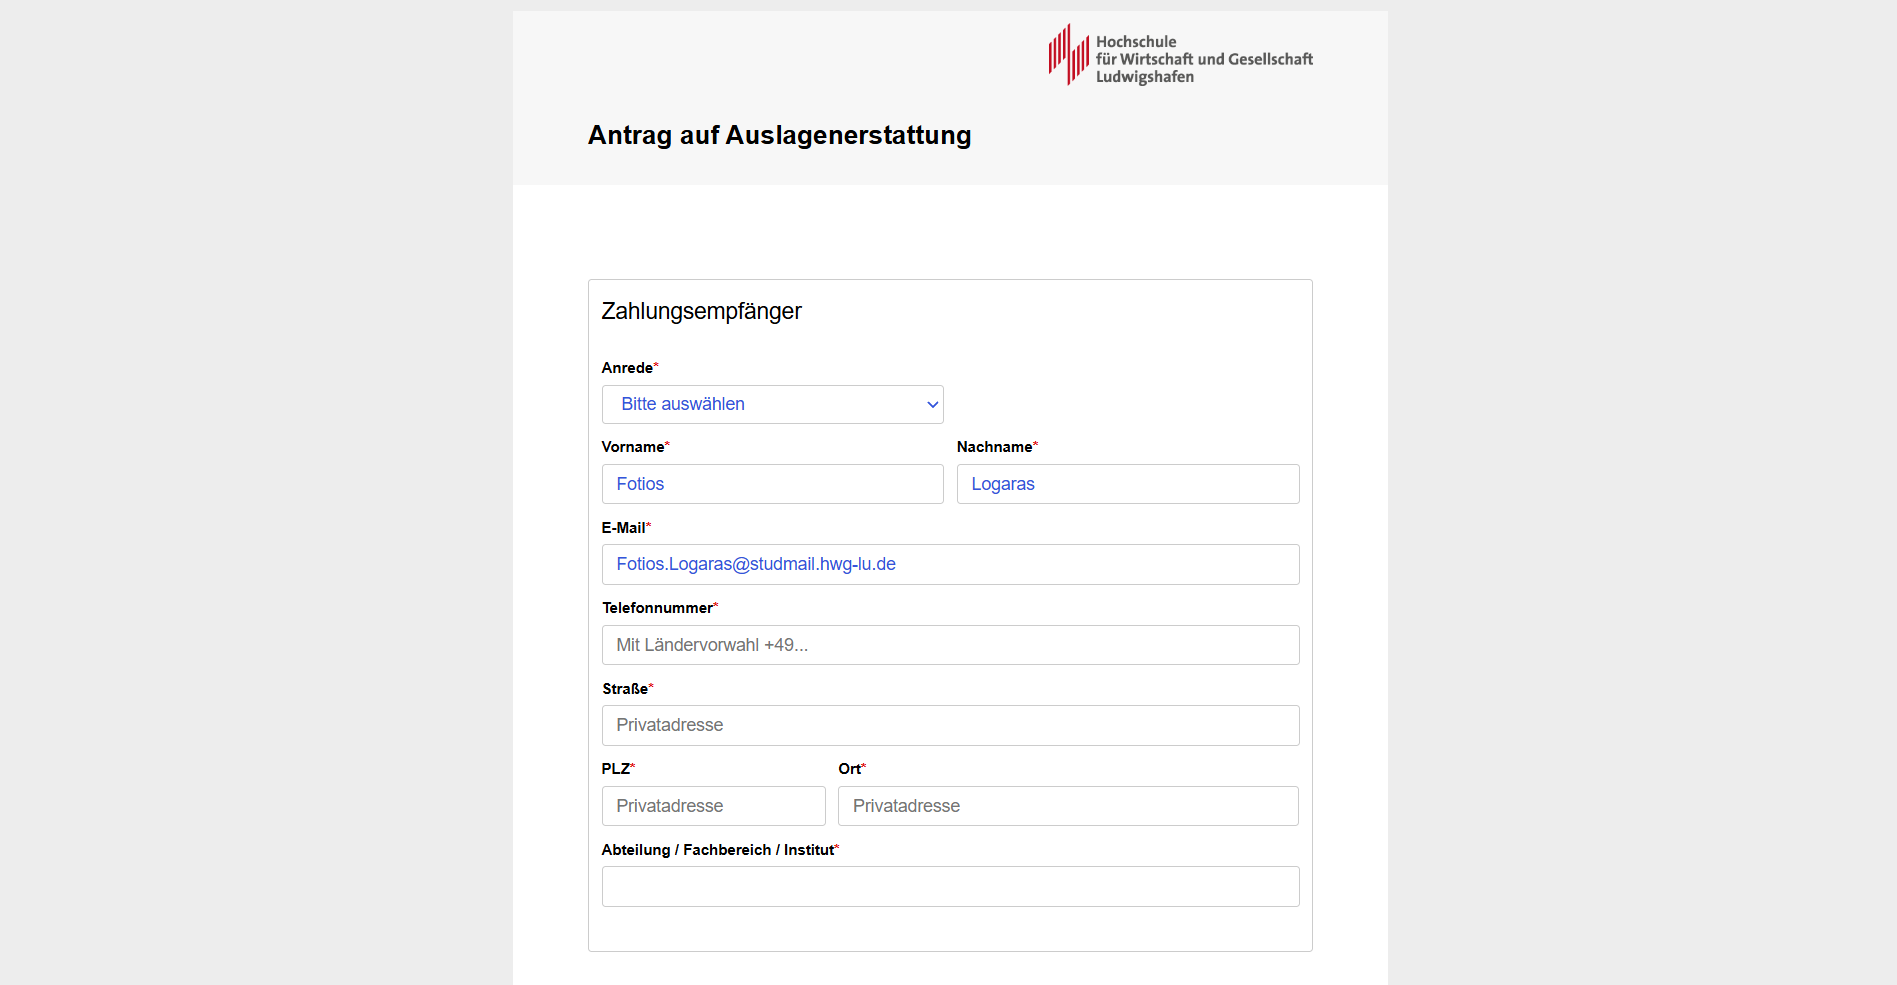
\includegraphics[width=\textwidth]{figures/Auslagenerstattung_Layout_Banner.png}
        \caption{Auslagenerstattung (700px, HWG-Logo)}
        \label{fig:header_auslagen}
    \end{subfigure}
    \hfill
    \begin{subfigure}[b]{0.48\textwidth}
        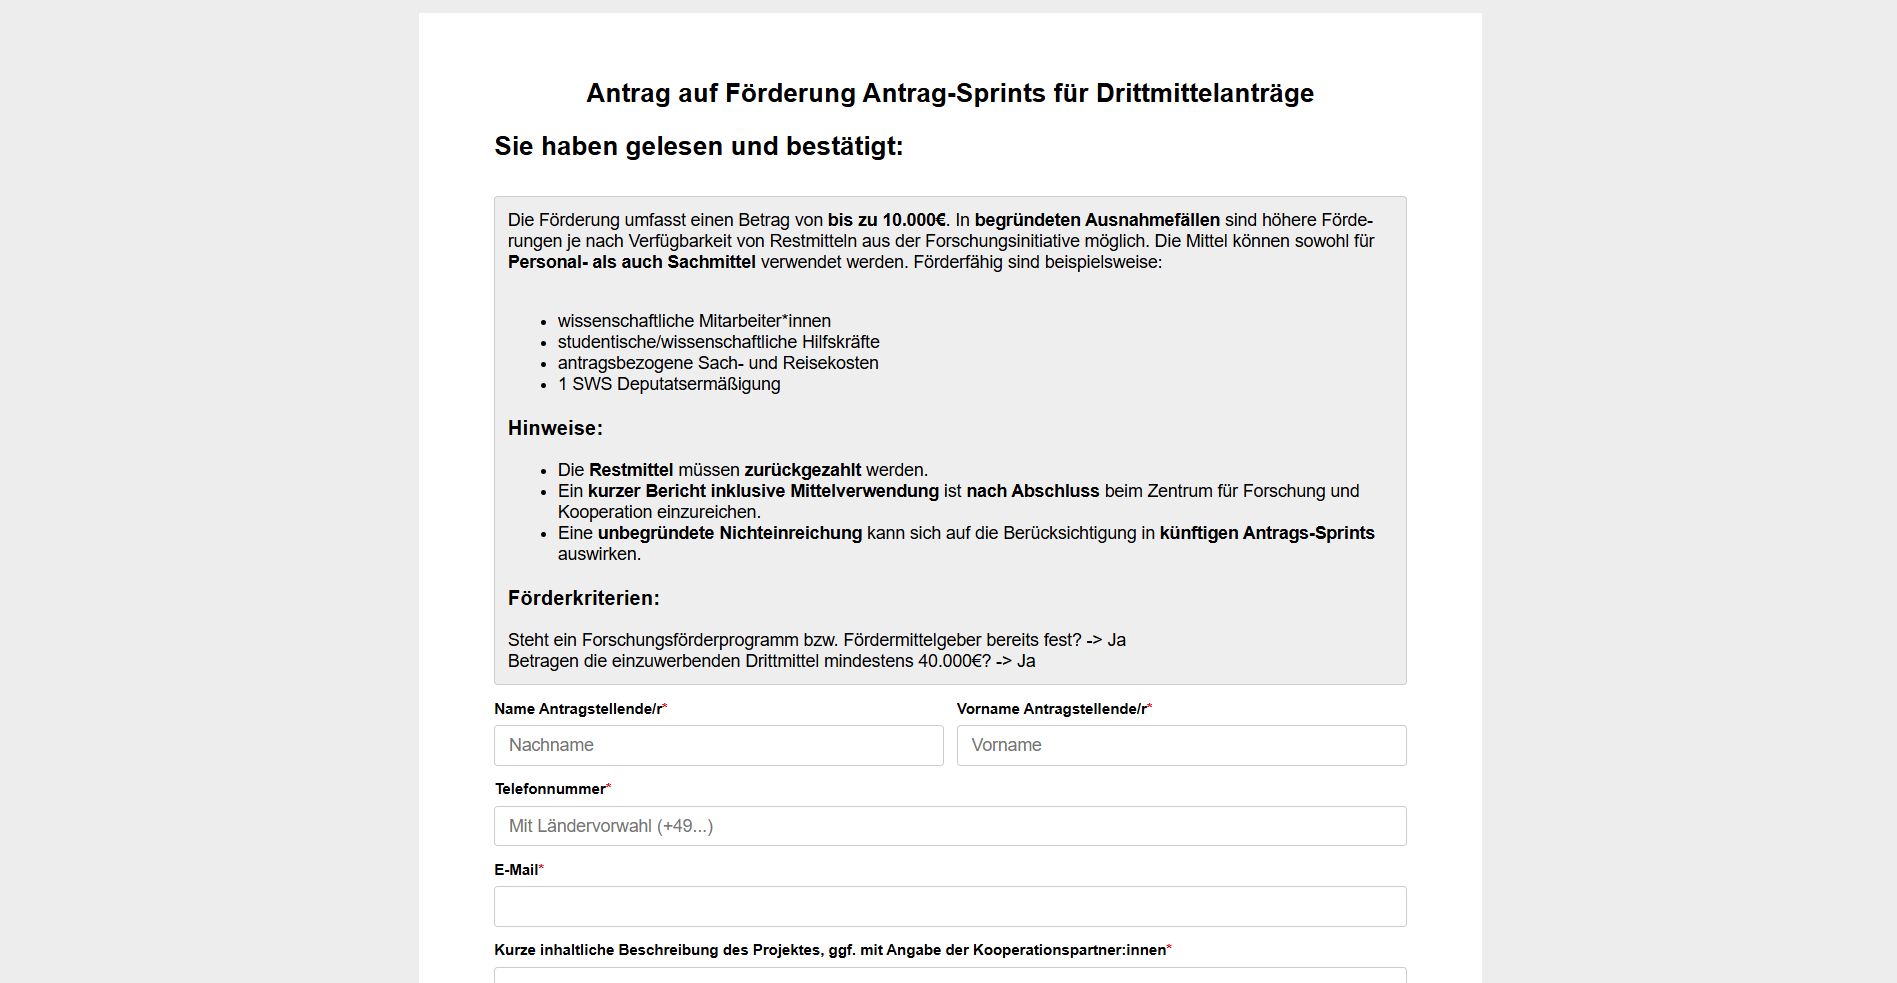
\includegraphics[width=\textwidth]{figures/Antrag_Sprints_Layout_Banner.png}
        \caption{Antrag-Sprints (850px, kein Logo)}
        \label{fig:header_sprints}
    \end{subfigure}
    \caption{Gegenüberstellung der Kopfbereiche und Corporate-Design-Elemente}
    \label{fig:vergleich_header}
\end{figure}

Darüber hinaus divergiert die Anordnung grundlegender Eingabefelder: Während im initialen Zahlungsempfänger-Block der \textit{Auslagenerstattung} (Abbildung~\ref{fig:header_auslagen}) intuitiv \textit{Vorname} links und \textit{Nachname} rechts angeordnet sind, kehrt Abbildung~\ref{fig:header_sprints} diese Reihenfolge in \textit{Name} (links) und \textit{Vorname} (rechts) um. Diese Permutation verstößt gegen die empirisch nachgewiesene Lesegewohnheit \parencite{bargas2010usable, wroblewski2008web}. Gleichwohl zeigt die spätere automatisierte Gesamtevaluation (Kapitel~\ref{chap:evaluation}), dass auch die \textit{Auslagenerstattung} über das gesamte mehrseitige Formular hinweg die Sequenz-Governance (\texttt{HWG-STAMM-01}) verletzt, da in nachgelagerten Abschnitten (z.\,B. Budgetverwaltung/Führungskraft) wiederholt persönliche Namens- und E-Mail-Felder nach der Telefonnummer eingeschoben werden. Ein weiteres CI-Defizit betrifft die Fußzeile: In 61\,\% der Vorlagen ist das herstellerseitige Werbelogo \textit{\enquote{Powered by XIMA Formcycle}} aktiv geschaltet.

\subsection{Problemfeld 3: Heterogene Stammdaten-Muster und Copy-Paste-Risiken}
\label{subsec:problem_stammdaten}

An der HWG existiert ein sogenanntes \textit{Master-Formular}, welches als wiederverwendbares Komponenten-Snippet zur Erfassung persönlicher Angaben konzipiert wurde. Da dieses Snippet jedoch nicht zentral als versionierte Bibliothek eingebunden, sondern von Erstellenden manuell kopiert und im Designer modifiziert wird, entstehen gravierende Inkonsistenzen:

\begin{figure}[htbp]
    \centering
    \begin{subfigure}[b]{0.48\textwidth}
        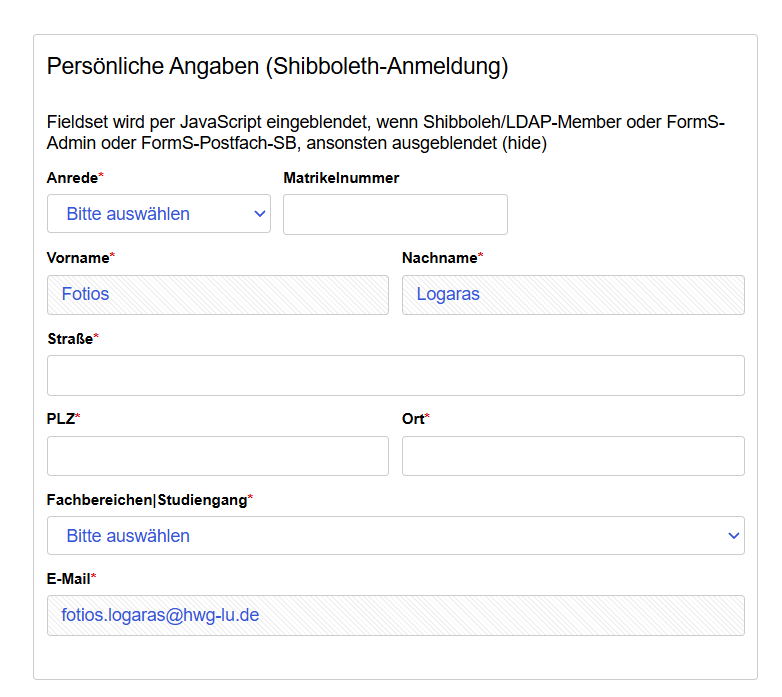
\includegraphics[width=\textwidth]{figures/Master_Formular_Persoenliche_Angaben.png}
        \caption{Master-Formular (Vorlage)}
        \label{fig:master_pers}
    \end{subfigure}
    \hfill
    \begin{subfigure}[b]{0.48\textwidth}
        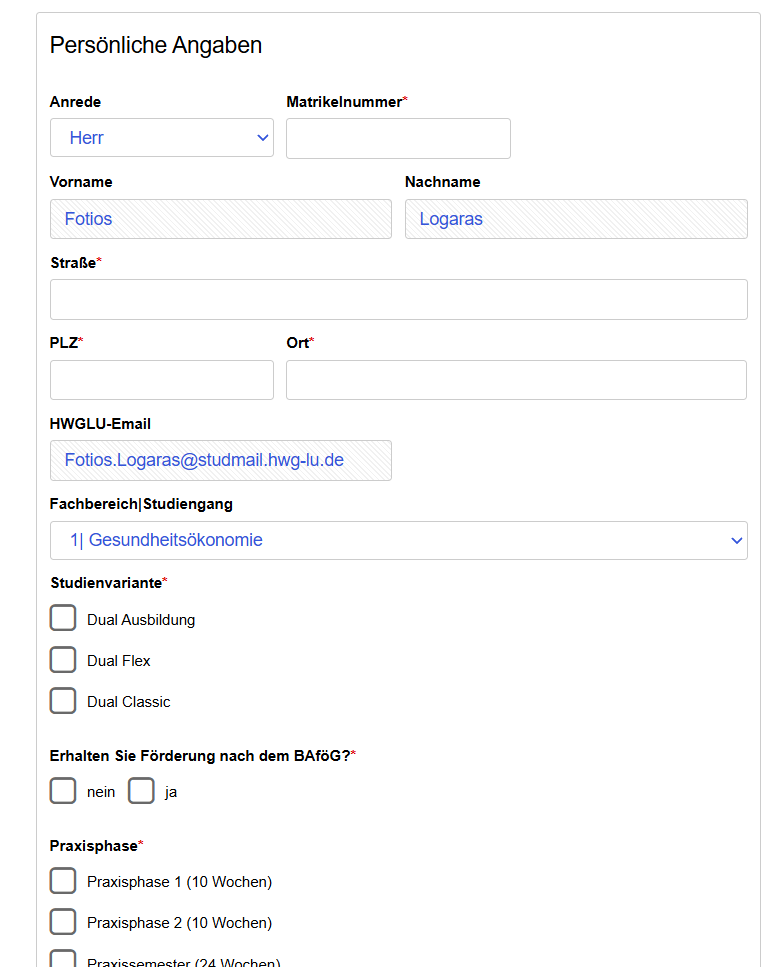
\includegraphics[width=\textwidth]{figures/FB1_Praktikum_Persoenliche_Angaben.png}
        \caption{FB1-Praktikumsantrag (Abwandlung)}
        \label{fig:praktikum_pers}
    \end{subfigure}
    \caption{Inkonsistenzen bei der Erfassung persönlicher Stammdaten}
    \label{fig:vergleich_stammdaten}
\end{figure}

Wie der Vergleich in Abbildung~\ref{fig:vergleich_stammdaten} belegt:
\begin{itemize}
    \item Im \textit{Master-Formular} (Abbildung~\ref{fig:master_pers}) sind \textit{Anrede*}, \textit{Vorname*}, \textit{Nachname*} und \textit{E-Mail*} als Pflichtfelder markiert; die \textit{Matrikelnummer} ist optional.
    \item Im \textit{FB1-Praktikum} (Abbildung~\ref{fig:praktikum_pers}) fehlen die Pflichtfeldsterne bei Name und E-Mail im DOM vollständig, während die \textit{Matrikelnummer*} zwingend gefordert wird.
    \item Das E-Mail-Feld variiert in der Beschriftung willkürlich zwischen \textit{E-Mail-Adresse}, \textit{E-Mail} und internen Bezeichnern wie \textit{HWGLU-Email}.
    \item Zudem enthält die Kopiervorlage im Designer-Produktivzustand sichtbare Entwickler-Notizen (\textit{\enquote{Fieldset wird per JavaScript eingeblendet, wenn Shibboleth/LDAP-Member authentifiziert}}), die für Endnutzende unverständlich sind und die \textbf{Selbstbeschreibungsfähigkeit (ISO 9241-110)} verletzen. Während dieser Hinweis im Vorlagen-Formular als beschreibender Rich-Text-Container (\texttt{rtevalue}) hinterlegt ist und in der automatisierten Einzelfall-Evaluation von Kapitel~\ref{chap:evaluation} mangels Label-Zuordnung keinen Punkteabzug auslöst, stellt ein solches Überbleibsel in abgeleiteten Anträgen ein kritisches Usability-Risiko dar (\texttt{HWG-UI-01}).
\end{itemize}

\subsection{Problemfeld 4: Schaltflächen-Semantik und die Fallstudie \enquote{Kritischer Fall}}
\label{subsec:problem_buttons}

Die Beschriftung von Aktionsschaltflächen (Microcopy) folgt keinen einheitlichen Regeln. Es finden sich uneinheitliche Mischformen aus kleingeschriebenen Minimal-Labels (\texttt{senden}), englischen Begriffen (\texttt{Submit}) und formalen Aktionsverben (\texttt{Antrag einreichen}, siehe Abbildung~\ref{fig:buttons_beispiele}): Während Abbildung~\ref{fig:btn_sprints} ein kleingeschriebenes Minimal-Label neben dem unklaren Ausnahmeknopf zeigt, illustriert Abbildung~\ref{fig:btn_kibeschaffung} eine abweichende Navigationsbeschriftung.

\begin{figure}[htbp]
    \centering
    \begin{subfigure}[b]{0.45\textwidth}
        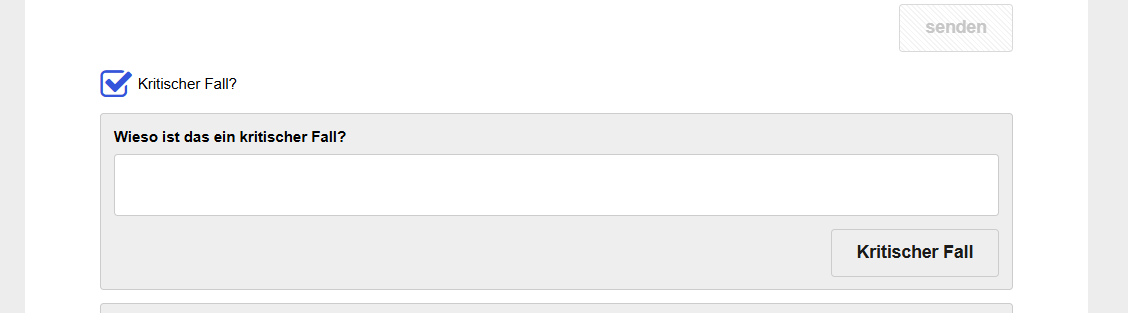
\includegraphics[width=\textwidth]{figures/Antrag_Sprints_Button.png}
        \caption{Antrag-Sprints (Minimal-Label \& Weiche)}
        \label{fig:btn_sprints}
    \end{subfigure}
    \hfill
    \begin{subfigure}[b]{0.45\textwidth}
        
\includegraphics[width=\textwidth]{figures/KI-Beschaffung_Button.png}
        \caption{KI-Beschaffung (Navigation)}
        \label{fig:btn_kibeschaffung}
    \end{subfigure}
    \caption{Heterogene Schaltflächen-Gestaltung im HWG-Bestand}
    \label{fig:buttons_beispiele}
\end{figure}

Ein besonders aufschlussreiches Usability-Phänomen offenbart die Fallstudie des Buttons \textit{\enquote{Kritischer Fall}}:

\textbf{Fachlicher Hintergrund \& Problemursache:} Im Zentrum für Forschung und Kooperation (ZFK) bestand die Anforderung, bei Förderanträgen mit außergewöhnlicher Tragweite eine gesonderte Prüfschleife unter Beteiligung des Hochschulpräsidenten einzuschalten. Anstatt diese Ausnahmeverzweigung organisatorisch in den nachgelagerten Prüf-Workflow einzubetten, verlagerten die Formularautoren die Weiche direkt in das Antragsformular: Sobald Antragstellende eine Checkbox aktivieren, wird der reguläre Absende-Button durch einen Button namens \textit{\enquote{Kritischer Fall}} ersetzt.

\textbf{Ergonomische Bewertung:} Aus Sicht der Dialoggestaltung nach \textcite{wroblewski2008web} und DIN EN ISO 9241-110 stellt dies einen gravierenden Bruch der \textbf{Erwartungskonformität} dar:
\begin{itemize}
    \item Ein Button muss zwingend dem \textbf{Action-Verb-Pattern} folgen (\textit{[Zielobjekt] + [Vollverb im Infinitiv]}). Die Beschriftung \textit{\enquote{Kritischer Fall}} ist ein reines Substantiv, das einen Ausnahmezustand beschreibt, jedoch keine Aktion.
    \item Antragstellende werden massiv verunsichert, ob sie einen Antrag einreichen oder einen Systemfehler melden.
    \item Eine fachliche Ausnahmeroute muss organisatorisch getrennt werden: Antragstellende betätigen stets \textit{\enquote{Antrag einreichen}}; die Sachbearbeitung leitet den Vorgang in der Prüfphase über eine rollenspezifische Schaltfläche an den Präsidenten weiter.
\end{itemize}

\subsection{Problemfeld 5: Defizite bei Barrierefreiheit und Eingabevalidierung}
\label{subsec:problem_a11y}

Die automatisierte DOM-Auswertung der gerenderten HTML-Dateien deckt erhebliche Mängel bezüglich digitaler Barrierefreiheit auf:
\begin{itemize}
    \item \textbf{Fehlen semantischer Gruppen (\texttt{<fieldset>}):} In 65\,\% der Formulare verzichten die Autoren auf \texttt{<fieldset>}-Tags mit \texttt{<legend>} und nutzen stattdessen rein visuelle \texttt{<div>}-Container. Für Screenreader geht dadurch der thematische Kontext von Eingabegruppen vollständig verloren (Verstoß gegen \textbf{WCAG 1.3.1}).
    \item \textbf{Inkonsistente ARIA-Attribute (\texttt{aria-required}):} In mehreren Vorlagen wird der Pflichtfeldstatus rein visuell über rote Sternchen signalisiert, ohne das maschinenlesbare Attribut \texttt{aria-required="true"} im Eingabeelement zu hinterlegen (\textbf{WCAG 3.3.2}).
    \item \textbf{HTML-Fragmente in Labels:} In 68\,\% der untersuchten Vorlagen enthalten die Label-Strings unmaskierte HTML-Tags (z.\,B. \texttt{<p>Vorname</p>} oder Entities wie \texttt{\&szlig;}). Dies führt bei Screenreadern zu störenden Ansagen.
\end{itemize}

\subsection{Problemfeld 6: Workflow-Fragmentierung und vertikale Abteilungssilos}
\label{subsec:workflow_silos}

Im Rahmen einer vertieften Untersuchung aller 49 im Korpus enthaltenen Workflow-Prozessgraphen wurde überprüft, ob hochschulweit standardisierte Prozessketten über mehrere Verwaltungseinheiten hinweg existieren. Die Datenanalyse der Prozessmodelle (\texttt{workflowVersions}) widerlegt dies:
\begin{itemize}
    \item \textbf{Hoher Anteil isolierter Einzelaufgaben:} Lediglich 14 der 49 Workflow-Prozessgraphen (29\,\%) binden zwei oder mehr Abteilungen bzw. Prüfinstanzen ein. Die Mehrheit (71\,\%) verbleibt als rein lokale Einzelaufgabe innerhalb einer spezifischen Organisationseinheit.
    \item \textbf{Vertikale funktionale Silos statt Querschnittsprozesse:} Wo mehrstufige Genehmigungsketten existieren, sind diese strikt fachdomänenspezifisch strukturiert (Personal, Finanzen, Forschung).
    \item \textbf{Inkonsistente Status-Nomenklatur:} Ein identischer Prozessschritt (\enquote{Genehmigung}) wird uneinheitlich als \textit{\enquote{Akzeptiert - VG}}, \textit{\enquote{Vergabe genehmigt}} oder \textit{\enquote{Antrag genehmigt}} bezeichnet. Zudem fehlen in vielen automatisierten E-Mails an Antragstellende eindeutige Vorgangsnummern (\texttt{[\%\$PROJECT\_ALIAS\%]}).
\end{itemize}

\section{Ableitung der Kernanforderungen an den Formular-Standard}
\label{sec:ableitung_anforderungen}

Aus der empirischen Ist-Analyse lassen sich fünf fundamentale Anforderungen ableiten:
\begin{enumerate}
    \item \textbf{Standardisierte Layout- und CI-Vorgaben:} Verbindliche Festlegung auf ein responsives Desktop-Raster (850px) sowie zwingende Einbindung des offiziellen HWG-Header-Banners und Deaktivierung herstellerseitiger Fußzeilen-Logos (\texttt{showlogo="0"}).
    \item \textbf{Zentrales Komponenten-Muster für Stammdaten:} Formalisierung eines verbindlichen Musters für persönliche Angaben mit fixer Feldabfolge (Anrede $\rightarrow$ Vorname $\rightarrow$ Nachname) und kanonischen Bezeichnungen.
    \item \textbf{Kontext- und rollenabhängige Microcopy-Regeln:} Zwingende Formulierung von Schaltflächen als handlungsorientierte Verben im Infinitiv (Action-Verb-Pattern); strikte Entkopplung von fachlichen Ausnahme-Workflows und primären Absende-Aktionen.
    \item \textbf{Regelbasierte Barrierefreiheits-Governance:} Maschinenlesbare Durchsetzung von \texttt{<fieldset>}-Strukturen sowie lückenlose Koppelung visueller Pflichtfeld-Sternchen an ARIA-Attribute.
    \item \textbf{Workflow-Harmonisierung und Prozesstransparenz:} Standardisierung der Lebenszyklus-Zustände, verbindliche Führung von Vorgangs-IDs in Bestätigungs-E-Mails sowie automatisierte Empfehlungen für Zwischenspeicher-Funktionen bei komplexen Mehrseiten-Anträgen.
\end{enumerate}
